\documentclass[letterpaper]{article}
\usepackage{aaai19}
\usepackage{times}
\usepackage{helvet}
\usepackage{courier}
\usepackage{url}
\usepackage{graphicx}
\frenchspacing

\nocopyright

\title{Polyp Segmentation Within Colonoscopy Images Using TernausNet V2}
\author{Soojin Jeon*, Eunsook Kang*, Hee Dong Yoon**, Yesol Cha**, Sangjun Oh***, and Young Sang Paik****\\
thezili.soojin@gmail.com\\
thezili.eunsook@gmail.com\\
yhd82@naver.com\\
petercha90@gmail.com\\
june@deepbio.co.kr\\
yspaik@gmail.com\\
\\
\*THE ZILI \ **Modulabs \ ***Deep Bio Inc. \ ****SK C&C
}

\begin{document}

\maketitle

\section{Introduction}

Colorectal cancer (CRC) is one of the leading causes among cancer deaths over the world. To reduce CRC mortality, it is a standard practive to screen polyps through regular colonoscopy. In foresight of the clinical need for a automatic support systems to aid the task, Gastrointestinal Image Analysis (GIANA) sub-challenge of the Endoscopic Vision Challenge organized by the International Conference On Medical Image Computing & Computer Assisted Intervention has provided an open dataset for polyp segmentation within colonoscopy images \cite{data1,data2,data3}. In this paper, we explore the effectiveness of TernausNet \cite{ternausnet}, the winning model of the Carvana Image Masking Challenge\footer{https://www.kaggle.com/c/carvana-image-masking-challenge}, in performing polyp segmentation using the given dataset.

\section{Method}

TernausNet is a binary segmentation model based on the U-Net architecture \cite{unet}, featuring a VGG11 \cite{vgg} encoder pretrained on the ImageNet dataset \cite{imagenet}. We trained this model on the 300 standard definition images and the 200 high definition images provided as the training set by \citeauthor{data1} \shortcite{data1}, \citeauthor{data2} \shortcite{data2}, and \citeauthor{data3}. The model was trained for 200 epochs with minibatch \cite{batch} of four, using binary cross entropy loss function, Adam \cite{adam} optimization, and cyclic learning rate.

\begin{figure}[h]
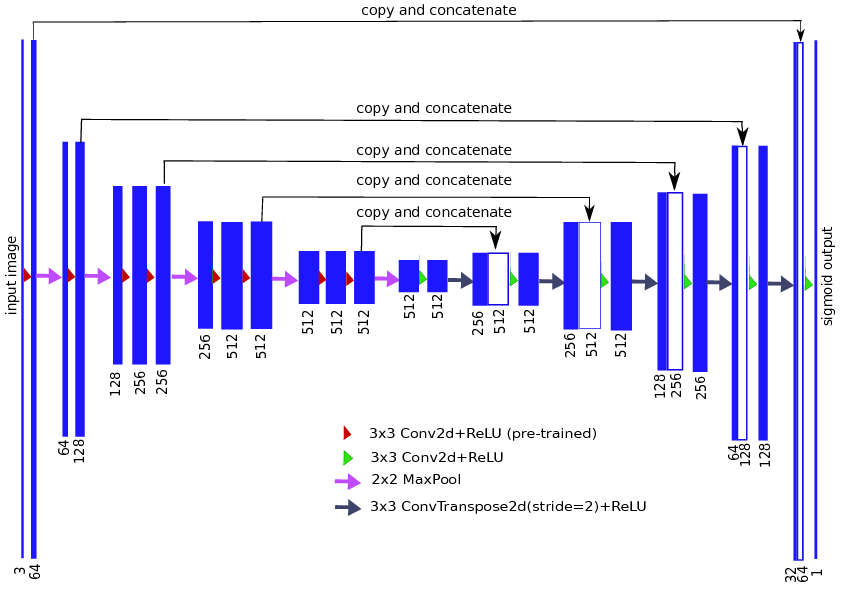
\includegraphics[width=8cm]{ternausnet.png}\centering
\caption{The TernausNet architecture.}
\end{figure}

In order to compensate for the small size of the training dataset, random affine transformations were used for data augmentation. Furthermore, additional segmentation masks were generated and trained along with the ground truth masks as pseudo labels \cite{pseudo}.

\section{Results}

DICE similarity score was used as the primary performance metric. After training on four GTX 1080TI GPUs with data parallelism applied, our model scored 0.94321 on the validation dataset.

\bibliography{main}
\bibliographystyle{aaai}

\end{document}
